% Crane horizontal-motion with hoist — Project Proposal
% Author: Caleb (drafted by GitHub Copilot)
\documentclass[11pt]{article}
\usepackage{amsmath,amssymb}
\usepackage{tikz}
\usepackage{siunitx}
\usepackage{geometry}
\geometry{margin=1in}
\title{Project Proposal: One-axis Gantry Crane with Autonomous Barrier-Overpass}
\author{Caleb Douglass \\ Draft prepared: \today}
\date{}

\begin{document}
\maketitle

\section*{Memo}
To: John Hedengren \\
From: Caleb K. D. \\
Date: \today \\
Re: Proposal for a single-axis gantry crane that detects an obstacle, raises the load to clear the obstacle, translates horizontally, then lowers the load.

This memo describes scope, sensors/actuators, models, risks, timeline and deliverables for the proposed control project.

\section{System description and block diagram}
The system is a small gantry/trolley that translates along one horizontal axis (x) on rails and includes a hoist that raises/lowers a payload (vertical coordinate $z$). A barrier (obstacle) may exist at fixed horizontal position(s) $x_b$ and height $h_b$. The controller senses the presence of the barrier and the load height using proximity sensors (ultrasonic or time-of-flight laser). The controller (ESP32 running MicroPython) commands two actuators: a horizontal drive (trolley motor) and a vertical hoist motor.

Key signals and variables:
- x(t): horizontal position of the trolley (m)
- z(t): vertical height of load relative to reference (m)
- m: mass of payload (kg)
- x_b, h_b: position and top height of barrier (m)
- u_x(t): command/force (or motor voltage) applied for horizontal motion
- u_z(t): command/force (or motor voltage) applied for vertical hoist
- y_b(t): barrier detection boolean / distance measurement
- y_z(t): measured load height from proximity sensor

Below is a schematic (not to scale).

\begin{center}
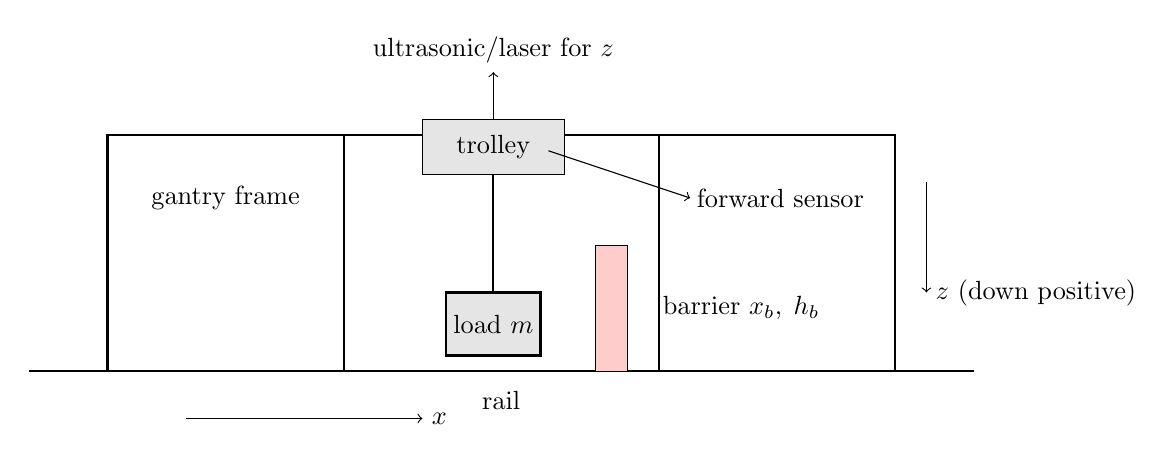
\begin{tikzpicture}[scale=1, every node/.style={scale=0.95}]
  % ground / rails
  \draw[thick] (0,0) -- (12,0) node[midway,below=4pt]{rail};

  % gantry supports
  \draw[thick] (1,0) -- (1,3) -- (4,3) -- (4,0);
  \draw[thick] (8,0) -- (8,3) -- (11,3) -- (11,0);

  % top beam
  \draw[thick] (4,3) -- (8,3);

  % trolley 
  \draw[fill=gray!20] (5.0,2.5) rectangle (6.8,3.2);
  \node at (5.9,2.85) {trolley};

  % hoist cable and load
  \draw[thick] (5.9,2.5) -- (5.9,1.0);
  \draw[thick,fill=black!10] (5.3,0.2) rectangle (6.5,1.0) node[midway]{load $m$};

  % barrier 
  \draw[fill=red!20] (7.2,0) rectangle (7.6,1.6);
  \node[right,xshift=10pt] at (7.6,0.8) {barrier $x_b,\; h_b$};

  % sensors
  \draw[->] (5.9,3.2) -- ++(0,0.6) node[above]{ultrasonic/laser for $z$};

  % forward sensor label
   \draw[->] (6.6,2.8) -- ++(1.8,-0.6) node[right,xshift=-1pt]{forward sensor};{forward sensor};

  % axes & variables
  \draw[->] (2, -0.6) -- ++(3,0) node[right]{$x$};
  \draw[->] (11.4, 2.4) -- ++(0,-1.4) node[right]{$z$ (down positive)};

  % gantry label remains
  \node at (2.5,2.2){gantry frame};

\end{tikzpicture}
\end{center}

\section{Objectives}
- Design and implement a controller on an ESP32 (MicroPython) to:
  1. Detect presence and height of a barrier at or near the trolley path.
  2. If the barrier obstructs the planned motion, raise the load to a safe clearance height $z_{\text{clear}} \ge h_b + \Delta$.
  3. Translate horizontally to the target position while maintaining safety limits.
  4. Lower the load to the nominal set point.
- Implement robust sensing (ultrasonic or time-of-flight laser) and filtering.
- Demonstrate reliable operation with a prototype and document results.

\section{Fixed factors (constants / parameters that cannot change during operation)}
- Gravitational acceleration $g \approx 9.81~\mathrm{m/s^2}$.
- Payload nominal mass $m$ (designized range; changing mass requires re-tuning).
- Geometry limits: rail length $L_{\text{rail}}$, maximum hoist travel $z_{\max}$ / minimum $z_{\min}$.
- Motor gear ratios, motor torque constants (nominal), power supply voltage (battery or bench).
- Sampling rate of MicroPython environment on ESP32 (practical upper bound due to interpreter and driver overhead).
- Mechanical friction/damping baseline (approximated as viscous coefficient $b_x,b_z$).

These constants will be measured or estimated and treated as parameters in the controller design.

\section{Actuator(s) and controllability}
Primary actuators:
- Horizontal drive motor (DC motor with gearbox or stepper) producing force/traction along $x$ (command $u_x$).
- Hoist motor for vertical motion (DC motor with gearbox or stepper) controlling $z$ (command $u_z$).

Controller implementability:
- Both actuators are directly commandable by the ESP32 (via motor drivers/PWM/H-bridge).
- The controller will implement closed-loop control loops for $x$ and $z$ (typically separate PID controllers with a simple higher-level state machine for barrier handling). If desired, trajectory pre-shaping (input shaping) or feedforward can be implemented to reduce oscillation.

Note: If the hoist is a wire cable and pendulum sway is significant, sway suppression techniques may be required; these increase control complexity and may require additional sensors (angle or accelerometers).

\section{Controlled variable(s) and setpoints}
- Primary controlled variables: $z(t)$ (load height) and $x(t)$ (horizontal position).
- Safety-critical requirement: when crossing a barrier at $x_b$, $z(t)$ must exceed clearance height $z_{\text{clear}}$ by a margin $\Delta$ (e.g., 50--100 mm).
- Performance requirements:
  - Achieve position setpoints within tolerance: $|x(t)-x_{\text{set}}| \le \epsilon_x$ (e.g., 5--20 mm).
  - Achieve height setpoints within tolerance: $|z(t)-z_{\text{set}}| \le \epsilon_z$ (e.g., 5--20 mm).
  - Minimize overshoot and avoid collisions.
- It is important to keep the load height within allowable range for safety and successful clearing. Secondary objective: minimize travel time while respecting motor limits.

\section{Dynamic model and equations}
We adopt a simplified 2-DOF point-mass model (no pendulum sway). This is appropriate for a stiff hoist (short cable) or rigid lifting attachment. More complex models (pendulum) are noted below.

Horizontal dynamics (Newton's law + viscous damping):
m \ddot{x}(t) + b_x \dot{x}(t) = F_x(t) = \alpha_x u_x(t)
where:
- m is payload mass (plus effective trolley inertia),
- b_x is viscous friction/damping along rail,
- u_x(t) is actuator command (e.g., applied motor voltage or current),
- \alpha_x maps command to force.

Vertical dynamics (hoist axis):
m \ddot{z}(t) + b_z \dot{z}(t) = F_z(t) - m g
or rearranged:
m \ddot{z}(t) + b_z \dot{z}(t) + m g = \alpha_z u_z(t)

If one includes motor electrical dynamics (for DC motor actuator with armature current i):
L \dot{i} + R i + K_e \omega = V (applied voltage)
\tau = K_t i
J \dot{\omega} + b_m \omega = \tau - \tau_{\text{load}}
and map motor torque to linear force through gearbox and drum radius.

Sensor models:
- Height sensor (ultrasonic or time-of-flight): y_z(t) = z(t) + n_z(t), with n_z zero-mean measurement noise; update rate f_s (e.g., 20--60 Hz).
- Barrier detector: returns either distance or boolean when distance < threshold. Possibility of false positives/negatives modeled by probability of detection P_D and false alarm P_FA.

Controller architecture (high level):
- State machine: IDLE $\rightarrow$ MOVE (if target) $\rightarrow$ DETECT\_BARRIER (on approaching region) $\rightarrow$ RAISE\_IF\_NEEDED $\rightarrow$ CROSS $\rightarrow$ LOWER\_TO\_SETPOINT.
- Low-level: PID or cascaded PID (position and velocity loops) on x and z axes; optional input shaping or feedforward for improved transient performance.

If cable pendulum dynamics are significant (single pendulum angle $\theta$ with length $\ell$), include:
\begin{align*}
m \ddot{x} + m \ell \ddot{\theta} \cos\theta - m \ell \dot{\theta}^2 \sin\theta + b_x \dot{x} &= F_x\\
\ell \ddot{\theta} + \ddot{x} \cos\theta + g \sin\theta + c_\theta \dot{\theta} &= 0
\end{align*}
These nonlinear equations motivate input-shaping or active anti-sway control.

\section{Sensors, sampling and control implementation}
Hardware planned:
- ESP32 microcontroller running MicroPython (control main loop, sensor drivers, communications).
- Motor drivers appropriate to chosen motors (DC or stepper drivers).
- Height sensor: either HC-SR04 ultrasonic sensor (inexpensive) or ST VL53L0X/VL53L1X time-of-flight laser sensors (better for narrow beams and reflective surfaces).
- Forward barrier detector: another ultrasonic or laser distance sensor oriented along travel direction.
- Optional IMU (accelerometer/gyro) to detect sway.

Software considerations:
- MicroPython provides ease of development; sample control loop at 20-200 Hz depending on complexity and sensor drivers.
- Implement PID controllers, low-pass filtering for sensors (e.g., complementary filter or simple exponential smoothing), debounce/verification logic for barrier detection.

\section{Factors influencing project success and risk mitigation}
Major risk areas:
1. Sensor reliability (false positive/negative barrier detection).
   - Mitigation: sensor fusion (use two sensor modalities if possible), filtering, threshold verification over multiple samples.
2. MicroPython timing/jitter/CPU limitations interfering with control loop deadlines.
   - Mitigation: profile loop performance, keep control loops light, potentially move tight loops to native code or use ESP-IDF/C if necessary.
3. Mechanical backlash, slop, or compliance causing positioning errors or sway.
   - Mitigation: include limit switches, calibrate encoders/position sensors, design mechanical pre-tensioning, speed limits.
4. Overloading motors or power supply issues.
   - Mitigation: select motors with margin, include current sensing and emergency stop, use proper PSU.
5. Pendulum sway if hoist cable is long.
   - Mitigation: keep cable short for prototype OR implement sway-damping strategies (input shaping, anti-sway control) and add IMU or angle sensors.
6. Safety / collision risk.
   - Mitigation: software soft-limits, physical bumpers, emergency stop button, watchdog.

Uncertain factors will be addressed by sequential testing: start with open-loop characterization (identify m, friction coefficients), then closed-loop position control on each axis, then integrate barrier logic and perform guided trials with slow speeds before increasing performance.

\section{Timeline and deliverables}
Proposed 5-week timeline (accelerated / semester mini-project):

- Week 1: Finalize detailed design and parts list; order components. Begin mechanical assembly of rails, trolley and hoist; create basic CAD/sketches and mount points.
- Week 2: Complete mechanical assembly and wiring. Integrate motor drivers and power; run basic open-loop motor tests and verify limit switches/encoders.
- Week 3: Integrate sensors on ESP32 (MicroPython): height sensor and forward detector drivers; implement simple filtering and validate measurements. Perform initial system identification (friction, travel limits).
- Week 4: Implement and tune low-level controllers (PID) for $z$ (hoist) and $x$ (trolley). Implement high-level state machine including barrier-detection and safe-raise logic. Add safety limits and emergency stop.
- Week 5: Robustness and corner-case testing, performance tuning, finalize documentation, capture demo video, and prepare final report and code repository.

Anticipated final product:
- Working prototype gantry that reliably detects a barrier and raises/lowers the load to clear it, along with source code (MicroPython), documentation, and a short demo video. A written final report in LaTeX summarizing design, models, experiments and results.

\section{Assessment metrics}
- Success rate of barrier clearing over N trials (target $>95\%$).
- Average time to perform barrier-overpass operation.
- Position and height tracking error statistics (RMS and max).
- Safety incidents: none.

\section{References}
The following references provide background on input-shaping, crane control, sensors and embedded platforms used in this project.

\begin{thebibliography}{9}
\bibitem{ogata}
K. Ogata, \emph{Modern Control Engineering}, 5th ed., Prentice Hall, 2010.

\bibitem{franklin}
G. F. Franklin, J. D. Powell, and A. Emami-Naeini, \emph{Feedback Control of Dynamic Systems}, 7th ed., Pearson, 2014.

\bibitem{singer-seering}
P. W. Singer and W. E. Seering, ``Preshaping command inputs to reduce system vibration,'' ASME Journal of Dynamic Systems, Measurement, and Control, vol. 112, no. 1, pp. 76--82, 1990.
% classic reference on input shaping / command shaping for cranes and flexible systems

\bibitem{esp32}
Espressif Systems, ``ESP32 Series Technical Reference Manual,'' Espressif, 2019. Available: \texttt{https://www.espressif.com/}

\bibitem{micropython}
MicroPython Developers, ``MicroPython Documentation,'' 2024. Available: \texttt{https://docs.micropython.org/}

\bibitem{vl53l0x}
STMicroelectronics, ``VL53L0X Time-of-Flight Ranging Sensor Datasheet,'' 2019. Available from STMicroelectronics.

\bibitem{hc-sr04}
HC-SR04 Ultrasonic Module Datasheet (commonly used sensor); many manufacturer datasheets are available online.

\end{thebibliography}

\section*{Notes and next steps}
This proposal frames the control problem, identifies sensors and actuators, gives compact dynamic equations and lists the risks and mitigations. Next steps (upon approval) are to finalize parts selection (motor torque, driver model, sensor models), order parts, and start the mechanical assembly and initial identification tests.

\end{document}
